% \VignetteIndexEntry{QTLBIM Overview}
% \VignetteDepends{qtlbim}
% \VignetteKeywords{QTL}
%\VignettePackage{qtlbim}
\documentclass{article}
\usepackage[margin=1in,head=0.5in,foot=0.5in]{geometry}



\usepackage{/unsup/R-2.4.0/lib/R/share/texmf/Sweave}
\begin{document}

\title{\textbf{QTL} Analysis using \textbf{B}ayesian \textbf{I}nterval \textbf{M}apping}
\author{Samprit Banerjee, Brian S. Yandell, William W. Neely, Nengjun Yi}
\maketitle



\abstract{
Bayesian interval mapping of QTL library R/qtlbim provides Bayesian
analysis of multiple quantitative trait loci (QTL) models. This
includes posterior estimates of the number and location of QTL, and of
their main and epistatic effects. This document assumes some
familiarity with QTL and with Bayesian methods. In addition it
provides graphical diagnostics that can help investigate several
"better" models. It also provides a 1-D and 2-D genome scan. 
The \texttt{R/qtlbim} package provides plotting facilities for results
generated by the analytical tools in the \texttt{R/qtlbim}
package. These plotting facilities include  time series plots of QTL
model charactacteristics as basic MCMC diagnostic plots, visual tools
for comparison of putative QTL models and exploratory plots whose
purpose is the aid in the identification of likely QTL.
This library R/qtlbim requires R/qtl 1.03.
}


\section{Overview}

\begin{Schunk}
\begin{Sinput}
> library(qtlbim)
> qb.load(hyper, qbHyper)
\end{Sinput}
\end{Schunk}

This vignette describes the MCMC sampling routines and some of the plotting
facilities available through the \texttt{R/qtlbim} package.  The
purpose of these plots is to provide graphical tools for 
\begin{enumerate}
\item exploring putative single and multiple QTL,
\item producing interpretable graphics of the relative evidence in
favor of a set of putative QTL,
\item visual diagnostics of the MCMC model selection algorithm.
\end{enumerate}  

This package is currently in "beta" release. That is, most of the
basic features are stable, but we expect a learning curve. We would
like feedback from experienced QTL mappers and R users
especially. Please note that the command \texttt{qb.mcmc} that creates
the MCMC samples produces external files in an output directory. These
files are tens of Mb large. They are integral to \texttt{R/qtlbim}
diagnostics. The proper way to remove a \texttt{qb} object created by
\texttt{qb.mcmc} is to use the \texttt{qb.remove} routine, as
indicated below. 

This document walks through the {\tt R/qtlbim} package by
demonstrating the following major functions: creation of Bayesian
samples from the posterior using MCMC sampling; use of plot and
summary tools to examine genetic architecture; data management in
R/qtlbim.


\section{Hyper Data Demo}

This document focuses on the \texttt{hyper} dataset
from \texttt{R/qtl}. 
One way to produce a \texttt{qb} object is to run
the \texttt{hyper} demo by typing
\begin{Schunk}
\begin{Sinput}
demo(qb.hyper.tour)
\end{Sinput}
\end{Schunk}
at the \texttt{R} prompt. 
Alternatively a \texttt{qb} object 
can be created by the  following sequence of commands. 
\begin{Schunk}
\begin{Sinput}
# First load the library
library(qtlbim)

# Now load the hyper data set.
data(hyper)

# Select just the columns in the hyper data set corresponding to  
# chromosomes one through 19.  This means that we have dropped
# the X-chromosome from our analysis, since R/qtlbim does not
# properly handle X yet.
hyper = subset(hyper, chr=1:19)

# Calculate genotype  probabilities.
hyper = qb.genoprob(hyper, step=2) 

# Now run the MCMC model selection algorithm. Running this command 
# may take as much as 15 minutes on slower computers.
qbHyper = qb.mcmc(hyper, pheno.col = 1, seed = 1616)
\end{Sinput}
\end{Schunk}

The comments in the code above describe the meaning of each step in
the sequence of commands used to produce \texttt{qbHyper}. The option
\texttt{seed} sets the random number seed so that this run can be
repeated exactly. The \texttt{demo(qb.hyper.tour)} or the 
\texttt{qb.mcmc} command above creates a \texttt{qb} object called
\texttt{qbHyper} that is used throughout this vignette.

\section{Bayesian QTL Mapping}

This section describes in more detail how to create Markov chain Monte
Carlo (MCMC) samples from the Bayesian posterior to be used for QTL
mapping.

The function {\tt qb.genoprob} creates a grid of putative QTL
positions throughout the entire genome and compute the genotypic
probabilities of the same. It would also compute genotypic
probabilities for missing markers. In general, the genotypes at
different loci are unobserved except at completely informative
markers but the probability distribution can be inferred from the
observed marker data using the multipoint method (\textsc{Jiang} and
\textsc{Zeng} 1997).

In the simplest case, where defaults in the next subsections are used,
MCMC samples are created with the following call:

\begin{Schunk}
\begin{Sinput}
qbHyper <- qb.mcmc(hyper, pheno.col = 1)
\end{Sinput}
\end{Schunk}

Named arguments to {\tt qb.data} and {\tt qb.model}, described in the
next two subsections, can be passed through {\tt qb.mcmc}. Otherwise,
default values are used. The next subsections detail the {\tt
qb.data}, {\tt qb.model} and {\tt qb.mcmc} routines.


\subsection{Specifying data}

The function {\tt qb.data} specifies the traits to be analyzed, their underlying
distribution, the random and/or fixed covariates and whether to standardize or to
use a boxcox transformation. Note that, the cross object can have several phenotypes
and some of which could be used as covariates.


\begin{Schunk}
\begin{Sinput}
qbData <- qb.data(hyper, pheno.col = 1, trait = "normal",
  boxcox = F, standardize = F)
\end{Sinput}
\end{Schunk}

\subsection{Defining the model}

The function {\tt qb.model} defines the model which is a Cockerham
epistatic model. For mapping a  \textit{K+1} genotypes per loci,
there are \textit{K} main effects and $K^{2}$ epistatic effects. For
a backcross population with two segregating genotypes $b_{q}b_{q}$
and $B_{q}b_{q}$ at locus \textit{q} the coefficients are

$x_{iq1} = z_{iq} - 0.5\; \mbox{and} \;x_{iqq'1} = x_{iq1}x_{iq'1}$

where $z_{iq}$ denotes the number of $b_{q}$ alleles. For an
intercross derived from two inbred lines, there are three
segregating genotypes $ b_{q}b_{q},\; b_{q}B_{q}$ and $B_{q}B_{q}$.
The coefficients of the Cockerham model are as follows:

$$x_{iq1} = z_{iq} + 1,\; x_{iq2} = (1-x_{iq1})(1+x_{iq1})-0.5\; \mbox{and}\;
x_{iqq'1}=\left \{\begin{array}{cc}
               x_{iq1}x_{iq'1} & k=1 \\
               x_{iq1}x_{iq'2} & k=2 \\
               x_{iq2}x_{iq'1} & k=3 \\
               x_{iq2}x_{iq'2} & k=4
             \end{array} \right.
  $$

 It also specifies if epistasis is considered, the expected number
 of main effect QTLs ({\tt main.qtl}), the prior number of total QTLs on all
 chromosome which includes QTLs with only epistatic effect,
 the maximum number of QTLs allowed per chromosome. The maximum number of
 QTLs allowed per chromosome has a default of $l_{0}+3\sqrt{l_{0}}$ where
$l_{0}$ is {\tt main.qtl} in a non-epistatic and
 {\tt mean.qtl} in an epistatic model. The interval
between two flanking QTLs for each chromosome and the fixed
covariate(s) interacting with QTLs are also specified. Typically a
real data set has several traits which can be considered as
covariates. By setting the {\tt max.qtl=0} ( the maximum number of
QTLs allowed) a traditional Bayesian model selection can be
performed. This provides a more relevant and shorter set of
covariates. This set of covariates can then be used to for QTL
mapping. For our case, as we have only a couple of covariates, we
include both in the model. The {\tt main.qtl}
argument of the {\tt qb.model} function refers to the prior number
of main effect QTL. This is obtained generally from a previous
rudimentary non-Bayesian analysis. For example, R/qtl can be used to
analyze this data without epistasis and the number of QTLs detected
could be used as the prior number of QTLs.
 
\begin{Schunk}
\begin{Sinput}
qbModel <- qb.model(hyper, epistasis = TRUE, main.nqtl = 3, 
  interval = rep(5,nchr(cross)), chr.nqtl = rep(2,nchr(cross)),
  depen = FALSE, prop = c(0.5, 0.1, 0.05))
\end{Sinput}
\end{Schunk}

\subsection{Running MCMC}

The function {\tt qb.mcmc} creates MCMC samples on
the data and model specified. The results are saved in a specified
directory, default being the current directory ("."). The {\tt
genoupdate} parameter of the {\tt qb.mcmc} function should be switched on
when there are many missing marker genotypes, as for the {\tt hyper}
dataset. For our case, we have only 7\% of the marker genotypes
missing so we are not updating the genotypes. There are two choices of
the MCMC algorithm namely, Metropolis-Hastings algorithm and the Gibbs
sampler. The M-H algorithm samples from a proposal density
approximating the conditional posterior distributions whereas Gibbs
sampler samples directly from the conditional posterior
distribution. The M-H algorithm is a lot faster compared to the Gibbs
sampler. We would saving 3000 samples which is the default {\tt n.iter}. It 
is worth mentioning that {\tt n.iter} does not specify the total number samples
drawn from the posterior distribution but merely indicates the number of samples that would be saved and used for posterior analysis. The first {\tt n.burnin} samples are discarded to allow the chain to converge to the posterior distribution and after that every {\tt n.thin} sample is considered to reduce serial
correlation resulting in a total of {\tt n.burnin + n.iter*n.thin} samples drawn.

\subsection{Examining a \texttt{qb} Object}

Please note that the plot and summary routines in this package all use
the S3 generic method. That is, we create an object with a call to
\texttt{qb.xxx} and then plot it using the generic \texttt{plot}
command. Manual pages show the complete set of command and plot
options.

The \texttt{qbHyper} is an object of class \texttt{qb} to which we can
apply the generic \texttt{summary} or \texttt{plot} routines. We defer
plots to later sections. Here we show only the summary:

\begin{Schunk}
\begin{Sinput}
> summary(qbHyper)
\end{Sinput}
\begin{Soutput}
Bayesian model selection QTL mapping object qbHyper on cross object hyper 
had 3000 iterations recorded at each 40 steps
with 1200 burn-in steps.
MCMC runs saved in temporary directory
 /tmp/Rinst2188206948/qtlbim/external/Hyper.MCMC 
(use qb.remove to remove).
Trait bp ( 1 ) treated as normal .
Trait was not standardized.
Epistasis was allowed.
Prior number of QTL: 3 main, 6 total, with 13 maximum.
Minimum distance between QTL:
    1     2     3     4     5     6     7     8     9    10 
 5.36 13.00 12.90  3.91  6.31  6.67  9.08 13.80 14.20 18.30 
   11    12    13    14    15    16    17    18    19 
 6.05 13.90 13.30 17.00  5.79 10.30  4.47 11.70 18.60 
Maximum number of QTL:
 1  2  3  4  5  6  7  8  9 10 11 12 13 14 15 16 17 18 19 
21  7  4 19 13 10  5  5  4  4 13  4  4  4 10  5 10  3  3 
QTL by environment not allowed.
Interacting covariates: 0
Diagnostic summaries:
          nqtl   mean envvar varadd  varaa    var
Min.     2.000  97.42  28.07  5.112  0.000  5.112
1st Qu.  5.000 101.00  44.33 17.010  1.639 20.180
Median   7.000 101.30  48.57 20.060  4.580 25.160
Mean     6.543 101.30  48.80 20.310  5.321 25.630
3rd Qu.  8.000 101.70  53.11 23.480  7.862 30.370
Max.    13.000 103.90  74.03 51.730 34.940 65.220

Percentages for number of QTL detected:
 2  3  4  5  6  7  8  9 10 11 12 13 
 2  3  9 14 21 19 17 10  4  1  0  0 

Percentages for number of epistatic pairs detected:
pairs
 1  2  3  4  5  6 
29 31 23 11  5  1 

Percentages for common epistatic pairs:
 6.15  4.15   4.6   1.7 15.15   1.4   1.6   4.9  1.15  1.17 
   63    18    10     6     6     5     4     4     3     3 
  1.5  5.11   1.2  7.15   1.1 
    3     2     2     2     2 
\end{Soutput}
\end{Schunk}

\section{Plotting MCMC History}
The final command above produced the \texttt{qbHyper} object by running the MCMC 
model selection algorithm:
\begin{Schunk}
\begin{Sinput}
qbHyper = qb.mcmc(hyper, pheno.col = 1, genoupdate=TRUE)
\end{Sinput}
\end{Schunk}
  Consequently a logical first step in exploring the results
of the analysis is to examine this MCMC chain.  The plotting tools in 
\texttt{R/qtlbim} provide a method for visually inspecting the history of the 
MCMC run.   The command
\begin{Schunk}
\begin{Sinput}
plot(qb.coda(qbHyper))
\end{Sinput}
\end{Schunk}
shows a default view of the MCMC chain as a time series. Each iteration of 
the MCMC chain represents a single model; therefore, we can explore the 
history of the MCMC chain by plotting time series for relevant model features.  
The time series plotted by  \texttt{qb.coda} show the sampling histories for
\begin{enumerate}
\item number of QTL in each model model (\texttt{nqtl}),
\item mean phenotype according to each model (\texttt{mean}),
\item environmental variability under each model (\texttt{envvar}),
\item variance explained under each model (\texttt{var}) and
%\item heritability under each model (\texttt{herit}).
\end{enumerate}

It is possible to plot a different subset of the model characteristics above, by using the 
optional argument \texttt{variables} in the \texttt{qb.coda} function.  For example,
in order to view just the number of QTL (\texttt{nqtl}) and the model means, use the following command.  The results of the following command are
shown in Figure~\ref{figPlotQBCODA}.
\begin{Schunk}
\begin{Sinput}
plot(qb.coda(qbHyper, variables = c("nqtl","envvar")))
\end{Sinput}
\end{Schunk}
\begin{figure}
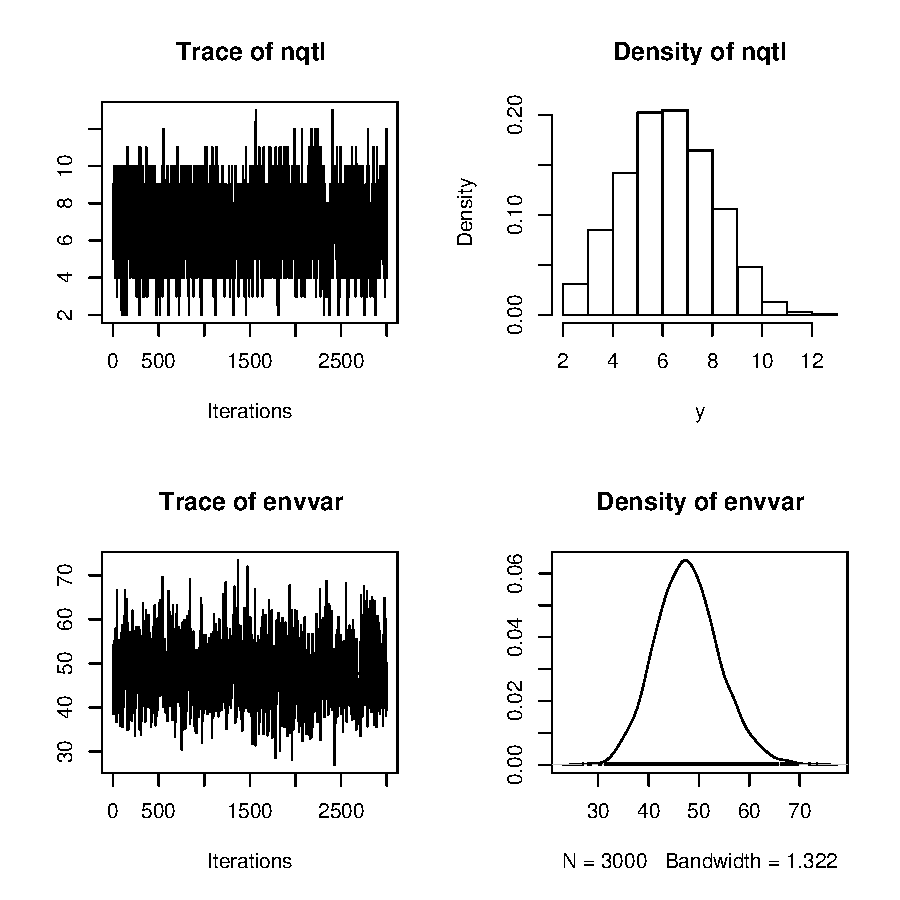
\includegraphics{qtlbimPDF/FIG-QBCODA}
\caption{Diagnostic Plot for a MCMC run.}
\label{figPlotQBCODA}
\end{figure}


\section{A Plot of QTL by chromosome}
From a biological perspective it may be interesting to view the location of possible QTL along 
the chromosome.  The function \texttt{qb.loci} shows a plot of quantitative 
trait loci for each chromosome.  The QTL are from single QTL models appearing as samples in the 
MCMC chain.  In the plot, the actual locations of possible QTL are jittered slightly in 
order to give a sense of the density of putative QTL in the vicinity of  each marker.  
The code
\begin{Schunk}
\begin{Sinput}
plot(qb.loci(qbHyper))
\end{Sinput}
\end{Schunk}
will produce a plot with all chromosomes. In order to view a subset of the 
chromosomes, the parameter \texttt{chr} to the generic \texttt{subset} routine can be used to limit the plot to a selected set 
of chromosomes.  The 
horizontal (blue) lines in the plot show the locations of markers.  
The markers themselves can be labelled by using the parameters 
\texttt{markers} in the function.
\begin{Schunk}
\begin{Sinput}
plot(qb.loci(subset(qbHyper, chr=c(3,4))), labels=TRUE)
\end{Sinput}
\end{Schunk} 
Figure~\ref{figPlotQBLOCI34} shows the result of this command.


\begin{figure}
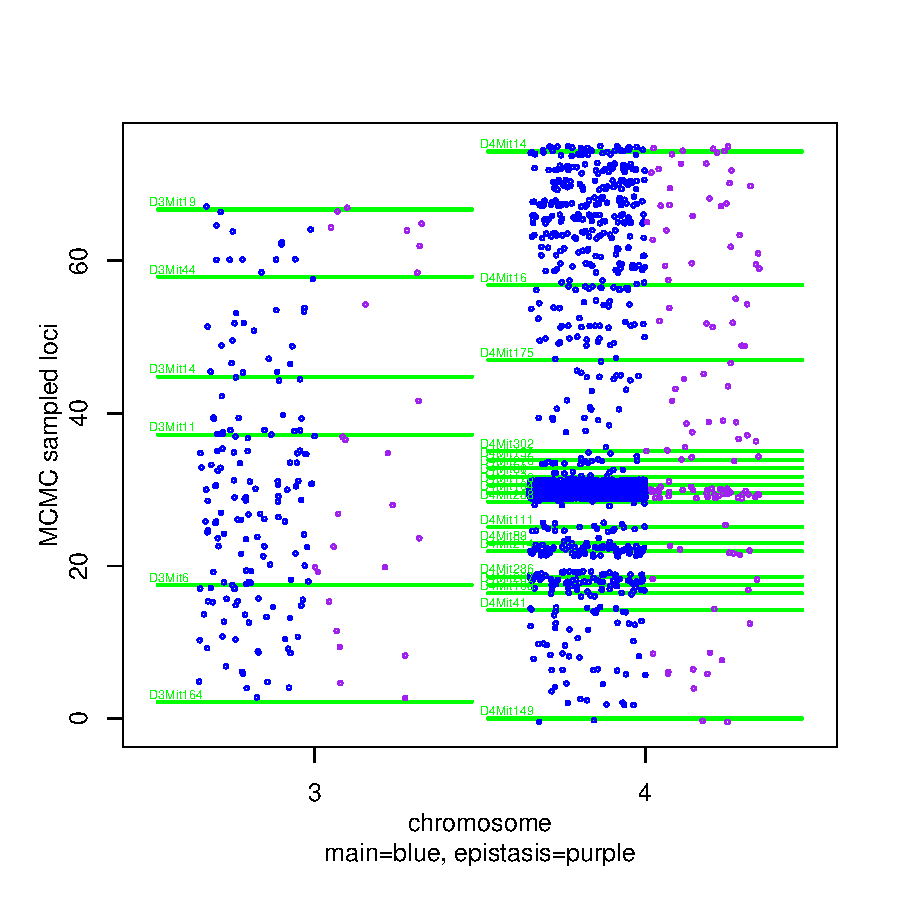
\includegraphics{qtlbimPDF/FIG-QBLOCI34}
\caption{A jittered plot of quantitative trait loci, showing only only chromosomes 3 and 4, with locations and marker labels.}
\label{figPlotQBLOCI34}
\end{figure}


\section{Summary Plots for Sampled Models}

The function \texttt{qb.BayesFactor} produces a composite (4-by-2) summary plot of the models 
sampled by the MCMC chain.  These plots are useful as an initial tool for examining the 
evidence in favor of multiple QTL models and in determining the locations of QTL. 
Figure~\ref{figPlotQBBF} shows the plot produced by the command 
\texttt{qb.BayesFactor(qbHyper)}.   The function of each of these plots is described below.
\begin{enumerate}
\item The plot appearing in the upper-left of the figure represents a
plot of the prior distribution for the number of QTL involved in
models (shown as a broken blue line) against the corresponding
posterior probabilities (shown as a histogram).
\item The plot in the upper-right shows Bayes factor ratios.  These
are the ratios of posterior probabilities to prior probabilities.  For
pairs of values along the horizontal axis of this plot, the member of
the pair with a larger Bayes factor ratio should be interpreted as
more likely. The vertical arrows give an indication of the strength of
evidence: weak (BF = 3), moderate (BF = 10) or strong (BF = 30).
\item The second row conveys information in terms of the  pattern of
chromosomes involved in the models.
\item The third row adresses the frequency of sampling each
chromosome.
\item The fourth row show relative importance of epistatic pairs. Here
the "6.15", or chr 6 by chr 15, epistatic pair is by far the strongest.
\end{enumerate}
\begin{figure}
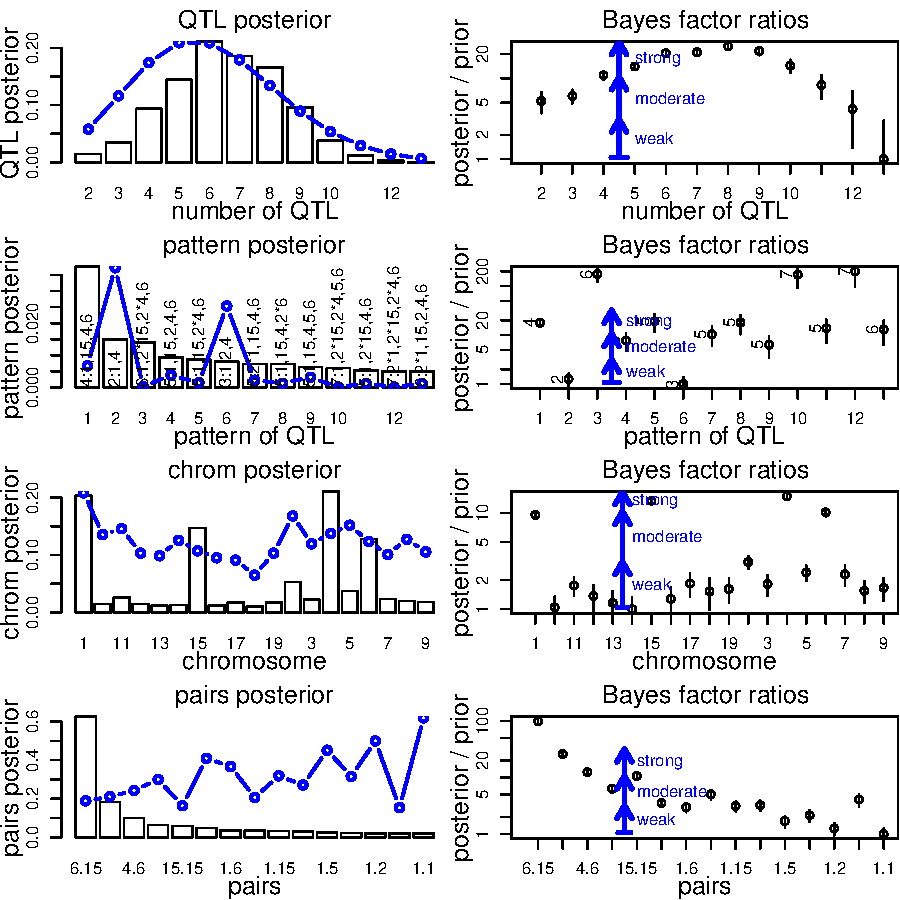
\includegraphics{qtlbimPDF/FIG-QBBF}
\caption{Paired plots of posteriors as bars overlaid by priors as blue
lines (left panels) with Bayes factor ratios to the least likely model
(right panels). Models in right panel can be compared by vertical
separation as scale is geometric. Blue arrows on right panels indicate
weak, moderate or strong Bayes factors for ratios of 3, 10 or 30,
respectively. Rows convey information about (1) number of QTL, (2)
chromosome pattern of QTL, (3) chromosomes, (4) epistatic pairs.}
strong 
\label{figPlotQBBF}
\end{figure}
As with other plot functions in the \texttt{R/qtlbim} package, it is
possible to limit attention of a subset of chromosomes using the
generic \texttt{subset} routine.  The \texttt{subset} argument
\texttt{pattern} can be used to limit the models plotted to those  
involving a specified list of chromosomes.  For example the command
\texttt{qb.BayesFactor(subset(qbHyper,pattern=c(2,3,17)))} considers
only those models involving chromosomes 2,3 and 17.  Repeats in the
pattern sequence indicate multiple QTL on the same chromosome.

\section{The Plot Demo}

The plot demo (\texttt{demo(qb.plot.tour)} gives a sample of the plots
available in the \texttt{R/qtlbim} package.  Running the plot demo
requires, the \texttt{lattice} package, which is loaded when you
attach the \texttt{R/qtlbim} package.
To start the plot demo, use the command 
\begin{Schunk}
\begin{Sinput}
demo(qb.plot.tour)
\end{Sinput}
\end{Schunk}

                   
The plot demo begins by giving a generic plot for the \texttt{qb} object
\texttt{qbHyper}. The \texttt{R/qtlbim} generic \texttt{qb} plot is
analogous to the generic \texttt{R} plot for linear model objects.
Where the generic plot for a linear model object shows a sequence of
graphics whose purpose is to aid in the initial results of model
fitting, the generic plot function for \texttt{qb} objects  shows  a
sequence of graphics whose purpose is to give an initial assessment of
the results produced by the MCMC algortihm. The generic plot for the
\texttt{qb} object \texttt{qbHyper} created above is shown with the 
command
\begin{Schunk}
\begin{Sinput}
plot(qbHyper)
\end{Sinput}
\end{Schunk}

The generic plot function shows a sequence of plots that include time
series plots of the mcmc chain, jittered plots of QTL by chromosome
and others.  The sequence of plots appearing in the plot demo is
listed below.

The list of plots shown by the generic plot function.
\begin{enumerate}
\item A time series plot of the mcmc chain runs.  This is shown in
Figure~\ref{figPlotQBCODA}, where it was
created by the command \texttt{plot(qb.coda(qbHyper))}. 
\item A jittered plot of QTL by chromosome.  This plot is identical to
the plot in Figure~\ref{figPlotQBLOCI} produced by the command
\texttt{plot(qb.loci(qbHyper))}. 
\item A model selection plot by chromosome.  This plot is identical to
\texttt{plot(qb.BayesFactor(qbHyper))} shown in Figure~\ref{figPlotQBBF}.
\item  Plot of QTL posterior for loci plus smooth estimates of QTL
effects.  This plot is the same as the plot generated by
\texttt{plot(qb.hpdone(qbHyper))}. 
Figure~\ref{figPlotQBHPD} shows the result of this command.
\item A plot of epistatic effects if such effects are
allowed. Figure~\ref{figPlotQBEPI} shows the result of the command
\texttt{plot(qb.epistasis(qbHyper))}. 
\item Summary diagnostics as histograms and boxplots by number of QTL.
This final diagnostic plot can be generated separately by the command
\texttt{plot(qb.diag(qbHyper))}. 
Figure~\ref{figPlotQBDIAG} shows the result of this command.
\end{enumerate}



\begin{figure}
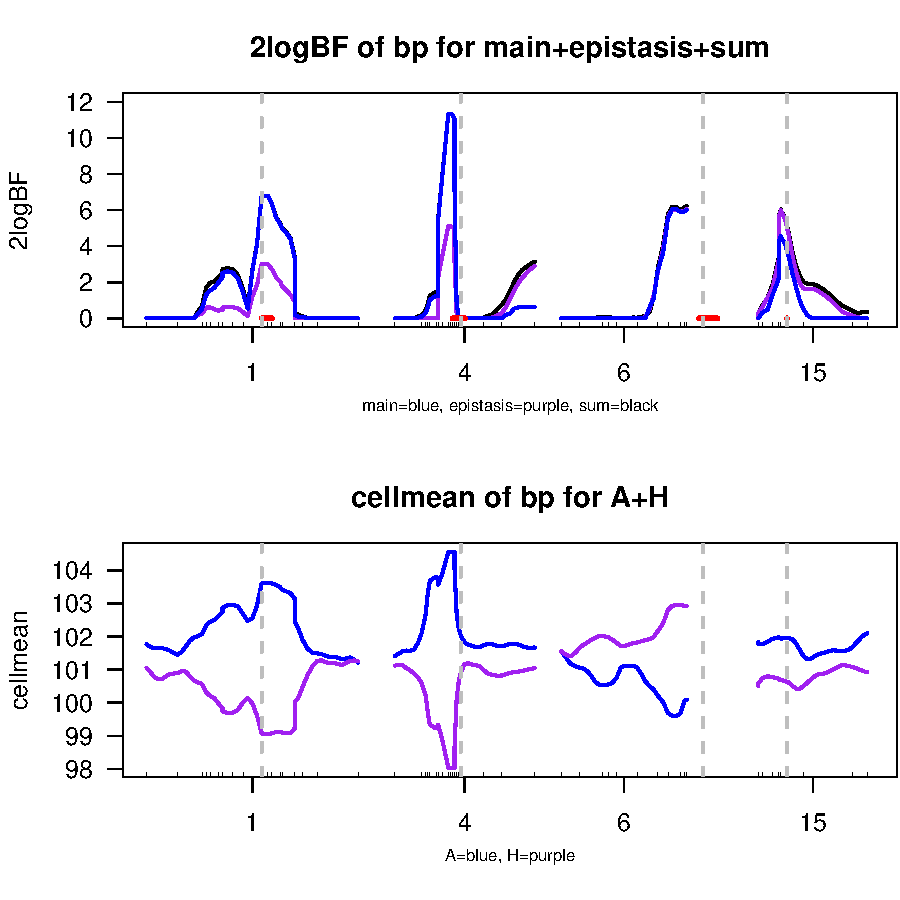
\includegraphics{qtlbimPDF/FIG-QBHPD}
\caption{A paired plot of posterior scan for loci above a scan of
marginal genotypic means by locus. In upper panel, black is overall
posterior, blue is for main effects and purple is for epistasis. In
lower panel, blue is for AA, purple for AB, and red for BB genotype at
scanned locus.}
\label{figPlotQBHPD}
\end{figure}


\begin{figure}
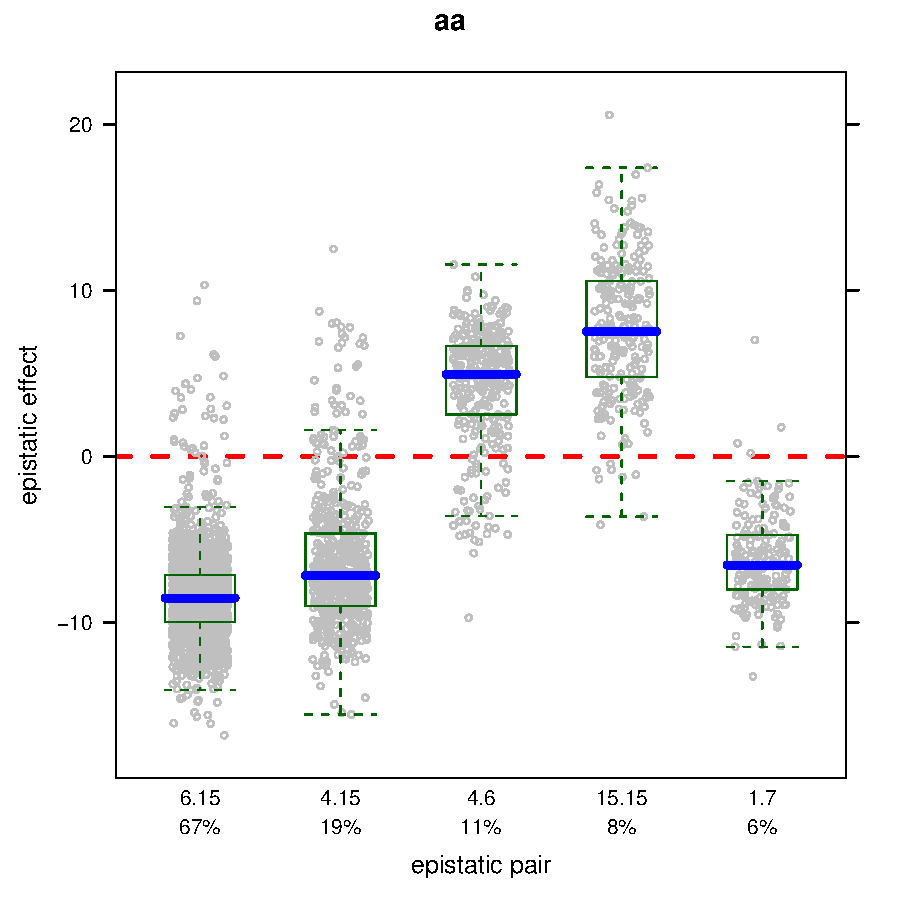
\includegraphics{qtlbimPDF/FIG-QBEPI}
\caption{A plot of epistatic effect by pair using Cockerham
effects. Only stronger epistatic pairs are shown. Blue line at median;
box contains 50\% of samples for epistatic pair. Percent below pair
indicates percent of MCMC samples with this epistatic pair.}
\label{figPlotQBEPI}
\end{figure}


\begin{figure}
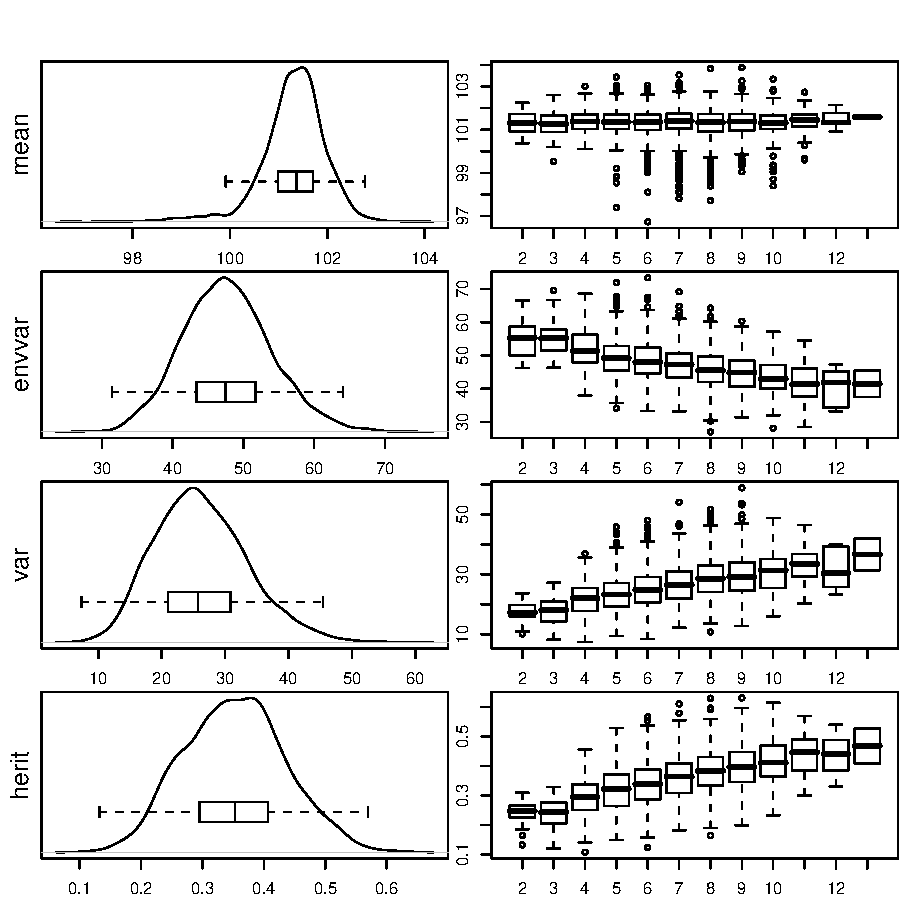
\includegraphics{qtlbimPDF/FIG-QBDIAG}
\caption{A set of diagnostic plots. Default has mean, unexplained
variance (\texttt{"envvar"}), explained variance (\texttt{"var"}), and
heritability (\texttt{"herit"}). Left panels show density plot and
horizontal box plot for all samples. Right panels show box plots by
number of QTL.}
\label{figPlotQBDIAG}
\end{figure}

\section{Data Management}

\subsection{Data Simulation}

R/qtlbim has an inbuilt function {\tt qb.sim.cross} to simulated a
backcross or F2 data set of class {\tt cross} (see R/qtl help pages
for details). The following chunk of code generates a data set of
100 individuals of F2 mating design. These individuals are genotyped
for 11 not equally spaced markers on 20 chromosomes. There are 7 QTLs,
two on chromosome 1 and one each on chromosomes 3,5,7,10 and 19. QTL
numbers 1,3 and 4 have additive main effects of 0.5, -0.5 and 0.5 and
numbers 2 and 4 have dominant main effects of 0.5 and -0.5. QTL
numbers 4 and 5 have an additive-additive interaction of -0.7 and
numbers 6 and 7 have an additive-dominant interaction of 1.2. Two
covariates, a binary fixed covariate and an ordinal random are
generated with their corresponding coefficients as 0.5 and 0.07. G x E
(gene x environemt) interaction is also considered with the fixed
covariate. A normal phenotype and an ordinal phenotype with 3
categories are measured. 7\% of the genotypes are randomly missing.

\begin{Schunk}
\begin{Sinput}
> cross <- qb.sim.cross(len = rep(100, 20), n.mar = 11, 
+     eq.spacing = F, n.ind = 100, type = "f2", 
+     ordinal = c(0.3, 0.3, 0.2, 0.2), missing.geno = 0.03, 
+     missing.pheno = 0.07, qtl.pos = rbind(c(1, 
+         15), c(1, 45), c(3, 12), c(5, 15), c(7, 
+         15), c(10, 15), c(12, 35), c(19, 15)), 
+     qtl.main = rbind(c(1, 0.5, 0), c(2, 0, 0.7), 
+         c(3, -0.5, 0), c(4, 0.5, -0.5)), qtl.epis = rbind(c(4, 
+         5, -0.7, 0, 0, 0), c(6, 8, 0, 1.2, 0, 
+         0)), covariate = c(0.5, 0.07), gbye = rbind(c(7, 
+         0.8, 0)))
\end{Sinput}
\end{Schunk}

By using the function {\tt qb.sim.cross} a list is attached to cross
object named "qtl".  This list is typically not a part of the {\tt
cross} object as described in {\tt read.cross} of the R/qtl library
and is generated only with the {\tt qb.sim.cross()} function.

\begin{Schunk}
\begin{Sinput}
> names(cross)
\end{Sinput}
\begin{Soutput}
[1] "geno"  "pheno" "qtl"  
\end{Soutput}
\end{Schunk}

The {\tt cross\$qtl} contains information about the true values
which can be compared to after the analysis.

\begin{Schunk}
\begin{Sinput}
> summary(cross$qtl)
\end{Sinput}
\begin{Soutput}
$pos
      chr pos
qtl.1   1  15
qtl.2   1  45
qtl.3   3  12
qtl.4   5  15
qtl.5   7  15
qtl.6  10  15
qtl.7  12  35
qtl.8  19  15

$herit.main
       qtl        add        dom
main.1   1 0.04653152 0.00000000
main.2   2 0.00000000 0.04560089
main.3   3 0.04653152 0.00000000
main.4   4 0.04653152 0.02326576

$herit.epis
       qtl.a qtl.b         aa         ad da dd
epis.1     4     5 0.04560089 0.00000000  0  0
epis.2     6     8 0.00000000 0.06700538  0  0

$herit.cov
   fix.cov    ran.cov 
0.02326576 0.02605765 

$herit.gbye
      qtl        add dom
GxE.1   7 0.02978017   0
\end{Soutput}
\end{Schunk}

The summary of the cross object summary is shown below.

\begin{Schunk}
\begin{Sinput}
> summary(cross)
\end{Sinput}
\begin{Soutput}
    F2 intercross

    No. individuals:    100 

    No. phenotypes:     4 
    Percent phenotyped: 96 94 92 95 

    No. chromosomes:    20 
        Autosomes:      1 2 3 4 5 6 7 8 9 10 11 12 13 14 15 16 17 18 19 20 

    Total markers:      220 
    No. markers:        11 11 11 11 11 11 11 11 11 11 11 11 11 11 11 11 11 11 11 11 
    Percent genotyped:  97.1 
    Genotypes (%):      AA:24.6  AB:50.6  BB:24.7  not BB:0  not AA:0 
\end{Soutput}
\end{Schunk}

\subsection{Cleaning Up}

Often we want to keep a \texttt{qb} object around for some time to
examine various diagnostics. While we might just use the \texttt{R}
command \texttt{rm} or \texttt{remove} to remove the internal object,
it is wise to instead use the \texttt{R/qtlbim} command
\texttt{qb.remove} to remove internal and external files. Recall that
\texttt{qb.mcmc} creates an external directory with a unique name,
containing tens of Mb of MCMC samples. The proper way to remove the
object \texttt{qbSim} is as follows:

\begin{Schunk}
\begin{Sinput}
qb.remove(qbSim)
\end{Sinput}
\end{Schunk}

[If you use \texttt{remove.qb} on qbHyper, you will also remove it
from your installed library, so be careful!]
It is possible to recover an orphaned external \texttt{qb} directory,
say if an \texttt{R} session is corrupted or the internal \texttt{qb}
object is inadvertantly removed. See the manual page on
\texttt{qb.recover} for further information.

\end{document}
